% Asset ID: FAS2DiscreteRandomVariablesTikZ-001
% Source: AI-proposed teaching enhancement based on lesson evidence
% Related lesson section: #8 Core Theory, #9 Visual Asset Integration, #15 Exam Technique Notes
% Used placeholder: FAS2DiscreteRandomVariablesTikZ-001
% Purpose: Provide a clean probability distribution calculation table template.

\documentclass[tikz,border=8pt]{standalone}
\usepackage{amsmath}
\usepackage{xcolor}
\usetikzlibrary{positioning,calc}
\definecolor{Canvas}{HTML}{FAF9F6}
\definecolor{Ivory}{HTML}{FFFFF0}
\definecolor{Line}{HTML}{E5E5EA}
\definecolor{Gold}{HTML}{C5A059}
\definecolor{SoftPink}{HTML}{FBEFEF}
\definecolor{Text}{HTML}{2C2C2E}
\begin{document}
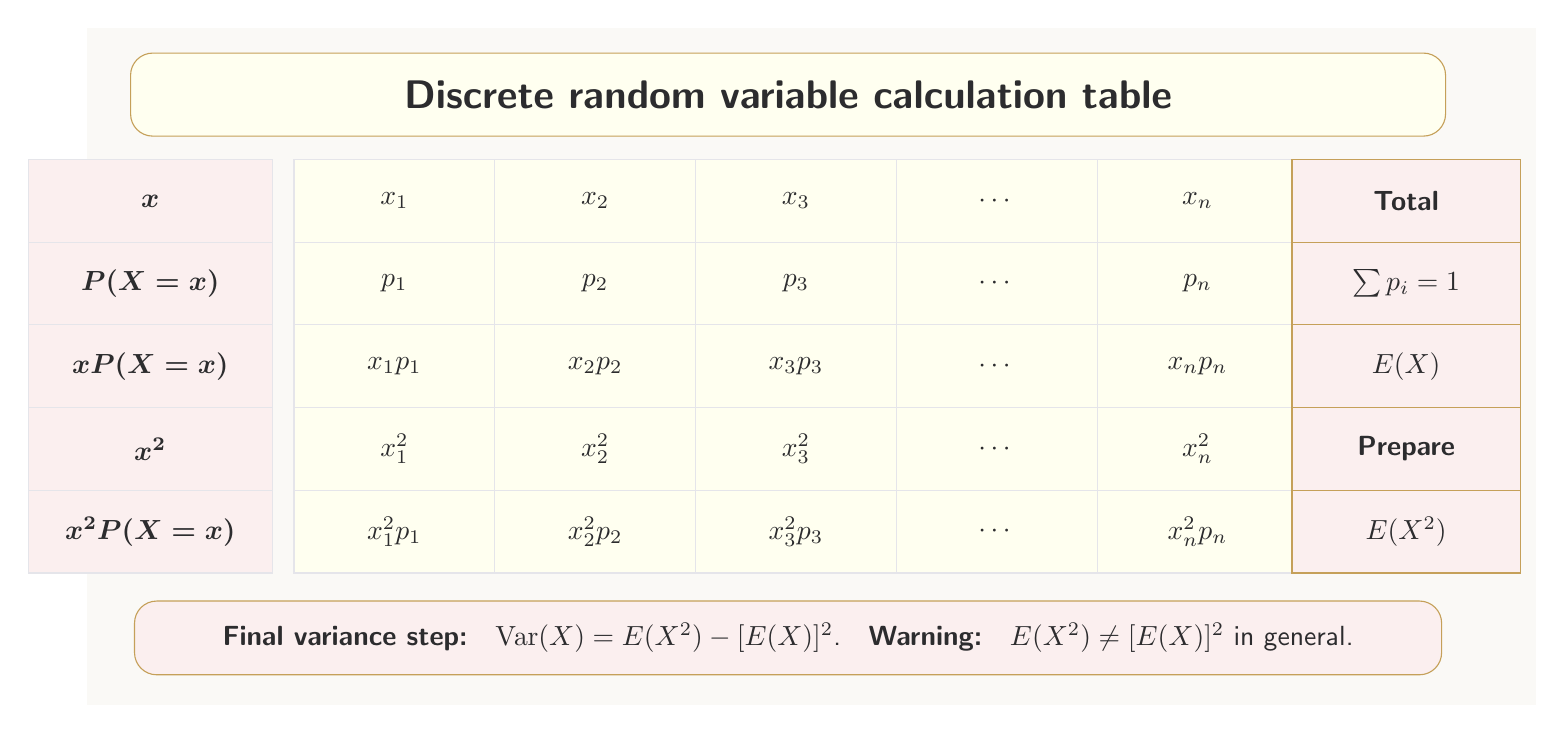
\begin{tikzpicture}[font=\sffamily,every node/.style={text=Text},cell/.style={draw=Line,minimum width=2.55cm,minimum height=1.05cm,align=center,fill=Ivory},labelcell/.style={draw=Line,minimum width=3.1cm,minimum height=1.05cm,align=center,fill=SoftPink,font=\sffamily\bfseries},totalcell/.style={draw=Gold,minimum width=2.9cm,minimum height=1.05cm,align=center,fill=SoftPink,font=\sffamily\bfseries}]
\fill[Canvas] (-0.8,-6.4) rectangle (17.6,2.2);
\node[draw=Gold,rounded corners=8pt,fill=Ivory,minimum width=16.7cm,inner sep=10pt] at (8.1,1.35) {\Large \textbf{Discrete random variable calculation table}};
\def\xlabel{0}\def\xa{3.1}\def\xb{5.65}\def\xc{8.2}\def\xd{10.75}\def\xe{13.3}\def\xtotal{15.95}
\def\yone{0}\def\ytwo{-1.05}\def\ythree{-2.10}\def\yfour{-3.15}\def\yfive{-4.20}
\node[labelcell] at (\xlabel,\yone) {$\boldsymbol{x}$};\node[cell] at (\xa,\yone) {$x_1$};\node[cell] at (\xb,\yone) {$x_2$};\node[cell] at (\xc,\yone) {$x_3$};\node[cell] at (\xd,\yone) {$\cdots$};\node[cell] at (\xe,\yone) {$x_n$};\node[totalcell] at (\xtotal,\yone) {Total};
\node[labelcell] at (\xlabel,\ytwo) {$\boldsymbol{P(X=x)}$};\node[cell] at (\xa,\ytwo) {$p_1$};\node[cell] at (\xb,\ytwo) {$p_2$};\node[cell] at (\xc,\ytwo) {$p_3$};\node[cell] at (\xd,\ytwo) {$\cdots$};\node[cell] at (\xe,\ytwo) {$p_n$};\node[totalcell] at (\xtotal,\ytwo) {$\sum p_i=1$};
\node[labelcell] at (\xlabel,\ythree) {$\boldsymbol{xP(X=x)}$};\node[cell] at (\xa,\ythree) {$x_1p_1$};\node[cell] at (\xb,\ythree) {$x_2p_2$};\node[cell] at (\xc,\ythree) {$x_3p_3$};\node[cell] at (\xd,\ythree) {$\cdots$};\node[cell] at (\xe,\ythree) {$x_np_n$};\node[totalcell] at (\xtotal,\ythree) {$E(X)$};
\node[labelcell] at (\xlabel,\yfour) {$\boldsymbol{x^2}$};\node[cell] at (\xa,\yfour) {$x_1^2$};\node[cell] at (\xb,\yfour) {$x_2^2$};\node[cell] at (\xc,\yfour) {$x_3^2$};\node[cell] at (\xd,\yfour) {$\cdots$};\node[cell] at (\xe,\yfour) {$x_n^2$};\node[totalcell] at (\xtotal,\yfour) {Prepare};
\node[labelcell] at (\xlabel,\yfive) {$\boldsymbol{x^2P(X=x)}$};\node[cell] at (\xa,\yfive) {$x_1^2p_1$};\node[cell] at (\xb,\yfive) {$x_2^2p_2$};\node[cell] at (\xc,\yfive) {$x_3^2p_3$};\node[cell] at (\xd,\yfive) {$\cdots$};\node[cell] at (\xe,\yfive) {$x_n^2p_n$};\node[totalcell] at (\xtotal,\yfive) {$E(X^2)$};
\node[draw=Gold,rounded corners=8pt,fill=SoftPink,minimum width=16.6cm,inner sep=8pt] at (8.1,-5.55) {\textbf{Final variance step:}\quad $\operatorname{Var}(X)=E(X^2)-[E(X)]^2$.\quad \textbf{Warning:}\quad $E(X^2)\neq [E(X)]^2$ in general.};
\end{tikzpicture}
\end{document}
